\chapter[Force and scenario centric]{Avoidance with criterion max $F_{c,y}$ as an exercise with both a scenario-centric and a force-centric perspective}
To determine the optimal avoidance for PM, the OCP presented in Chapter~\ref{cha:ch4} is used. The vehicle and the optimization properties are reused from Table~\ref{tab:num_sol_opt_avoid_PM_params}. 

The angle of the obstacle ($\psi_v$) is the angle between the component of the global force ($F_{x}$) and the velocity vector, and is calculated using 
\begin{align}
    \psi_v(t) &= \frac{dy(t)}{dx(t)}.
\end{align}
The vehicle centric control force vectors ($F_{c,x}$ and $F_{c,y}$) are calculated using
\begin{align}
    \begin{bmatrix}
        F_{v,x}(t) \\
        F_{v,y}(t)
    \end{bmatrix} &=
    \begin{bmatrix}
        \cos\left(\psi_v(t)\right) & \sin\left(\psi_v(t)\right) \\
        -\sin\left(\psi_v(t)\right) & \cos\left(\psi_v(t)\right)
    \end{bmatrix}
    \begin{bmatrix}
        F_{x}(t)\\
        F_{y}(t)
    \end{bmatrix}.
\end{align}
$\psi_v$ when the vehicle just touches the obstacle at time $t_o$ is calculated using 
\begin{align}
    \theta &= \psi_v(t_o)\vert_{f_o(x,y)=1}.
\end{align}
The scenario centric control force vectors ($F_{c,x}$ and $F_{c,y}$) are calculated using
\begin{align}
    \begin{bmatrix}
        F_{c,x}(t) \\
        F_{c,y}(t)
    \end{bmatrix} &=
    \begin{bmatrix}
        \cos\left(\theta\right) & \sin\left(\theta\right) \\
        -\sin\left(\theta\right) & \cos\left(\theta\right)
    \end{bmatrix}
    \begin{bmatrix}
        F_{x}(t)\\
        F_{y}(t)
    \end{bmatrix}.
\end{align}

The optimization results for the force and scenario centric are presented in Figure~\ref{fig:prob5_res}. From the figure, it is clear that the control force magnitude for the $y$ direction is constant for both the scenario-, vehicle-, and global-centric. However, the $x$ is different for scenarios, which is rather intuitive.

\vspace{5pt}
\noindent\fbox{%
    \parbox{\textwidth}{%
        \textbf{Some reflections}: \newline
        It is worth mentioning that, in Figures~\ref{fig:num_sol_opt_avoid_PM_res_pic} and ~\ref{fig:prob5_res}, the intersection occurs at $t = 1.07$s. However, the vehicle starts to decelerate in the $y$-direction at around 1\,s, when $x = 20$\,m. This is probably due to the order of sharpness of the obstacle. when the degree of the super ellipse (obstacle model) is reduced, the vehicle starts to decelerate earlier. 
    }%
}

\begin{figure}[h!]
    \centering
    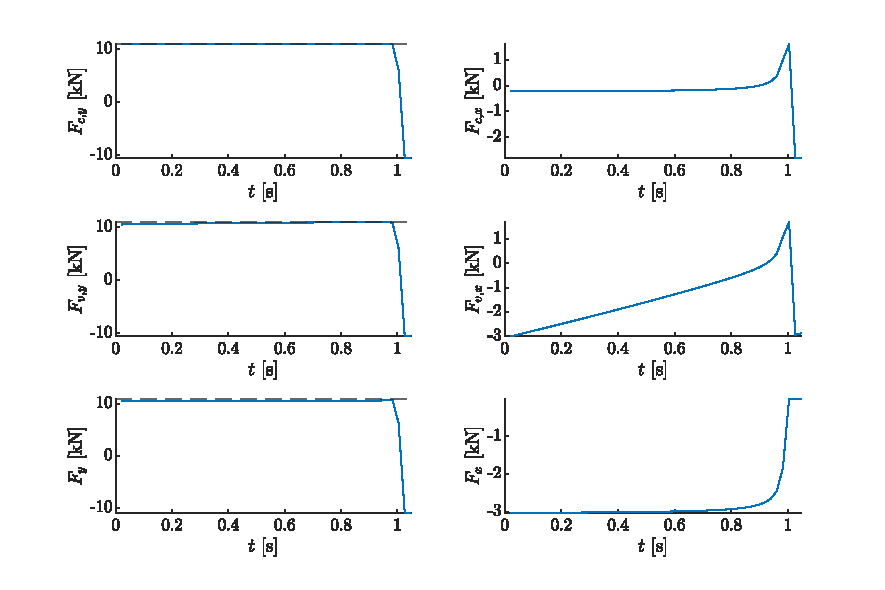
\includegraphics{figures/prob5_opt_avoid_controlforce.pdf}
    \caption{Criteria for max $F_{c,y}$ for both a scenario-centric and a force-centric perspective.}
    \label{fig:prob5_res}
\end{figure}

\subsection{Code}
The source codes for this problem can be found at \newline \href{https://github.com/arvba41/optimal_vehicle_maneuvers/blob/main/uppgift/ugf4/opti_veh_men_prt.m}{https://github.com/arvba41/optimal\_vehicle\_maneuvers}.